%%%%%%%%%%%%%%%%%%%%%%% file typeinst.tex %%%%%%%%%%%%%%%%%%%%%%%%%
%
% This is the LaTeX source for the instructions to authors using
% the LaTeX document class 'llncs.cls' for contributions to
% the Lecture Notes in Computer Sciences series.
% http://www.springer.com/lncs       Springer Heidelberg 2006/05/04
%
% It may be used as a template for your own input - copy it
% to a new file with a new name and use it as the basis
% for your article.
%
% NB: the document class 'llncs' has its own and detailed documentation, see
% ftp://ftp.springer.de/data/pubftp/pub/tex/latex/llncs/latex2e/llncsdoc.pdf
%
%%%%%%%%%%%%%%%%%%%%%%%%%%%%%%%%%%%%%%%%%%%%%%%%%%%%%%%%%%%%%%%%%%%


\documentclass[runningheads,a4paper]{llncs}

\usepackage{amssymb}
\setcounter{tocdepth}{3}
\usepackage{graphicx}

\usepackage{url}
\urldef{\mailsa}\path|{alfred.hofmann, ursula.barth, ingrid.haas, frank.holzwarth,|
\urldef{\mailsb}\path|anna.kramer, leonie.kunz, christine.reiss, nicole.sator,|
\urldef{\mailsc}\path|erika.siebert-cole, peter.strasser, lncs}@springer.com|    
\newcommand{\keywords}[1]{\par\addvspace\baselineskip
\noindent\keywordname\enspace\ignorespaces#1}

\begin{document}

\mainmatter  % start of an individual contribution

% first the title is needed
\title{Developing an object-oriented library in JavaScript to build modular and flexible cross-platform evolutionary algorithms}

%\title{Lecture Notes in Computer Science:\\Authors' Instructions
%for the Preparation\\of Camera-Ready
%Contributions\\to LNCS/LNAI/LNBI Proceedings}

% a short form should be given in case it is too long for the running head
\titlerunning{Developing an object-oriented library in JavaScript}

% the name(s) of the author(s) follow(s) next
%
% NB: Chinese authors should write their first names(s) in front of
% their surnames. This ensures that the names appear correctly in
% the running heads and the author index.
%

\author{V\'{\i}ctor M. Rivas\inst{1} \and Juan Juli\'{a}n Merelo\inst{2}}
%
%%%% modified list of authors for the TOC (add the affiliations)
\tocauthor{V\'{\i}ctor M. Rivas (Universidad de Ja\'{e}n),
Juan Juli\'{a}n Merelo (Universidad de Granada)}
%
\institute{Universidad de Ja\'{e}n, Ja\'{e}n, Spain,\\
%\email{},\\ WWW home page:\texttt{}
\and
Universidad de Granada, Granada, Spain}



%
\authorrunning{V.M. Rivas et al.}
% (feature abused for this document to repeat the title also on left hand pages)

% the affiliations are given next; don't give your e-mail address
% unless you accept that it will be published

%
% NB: a more complex sample for affiliations and the mapping to the
% corresponding authors can be found in the file "llncs.dem"
% (search for the string "\mainmatter" where a contribution starts).
% "llncs.dem" accompanies the document class "llncs.cls".
%

%\toctitle{Lecture Notes in Computer Science}
\maketitle

\begin{abstract}
This paper introduces a new distributed evolutionary computation system that uses the computational capabilities of the web browser. Using Asynchronous JavaScript allows anybody with a web browser
to participate in evolutionary experiments with little or none effort. Since, in
this case, computing becomes a social activity and is inherently unpredictable, in this paper we will explore the performance of this kind of virtual computer by solving two simple problems, such as the Royal Road function and a 128-terms equation, and analysing how many machines and evaluations it yields. We will also examine possible performance bottlenecks
and how to solve them, and, finally, issue some advice on how to setup
this kind of experiments to maximize turnout and, thus, performance.
This paper attempts to reproduce results of older papers using modern
browsers and all kind of devices that, nowadays, have JavaScript integrated in the browser, and is a complete rewrite of the code using the popular MooTools library. 
Results show that the system allows the rapid development of evolutionary algorithms, suited for different chromosomes representations and problems, that can be simultaneously executed in many different operating systems and web browsers, sharing the best solutions previously found.
\keywords{Web browser-based computation, Javascript library, asynchronous communication}
\end{abstract}

% no key words

\section{Introduction and state of the art}
\label{sec:intro}
% no \PARstart
Javascript language was introduced in Netscape Navigator in 1995, rapidly adopted by Microsoft's web browsers, and standardized for first time by ECMA International in 1997, with the name of ECMAScript. This interpreted language gave web navigators (but also e-mail clients) the power to perform some kind of computation apart from the needed to render HTML code.
Application--level networks (ALNs), are configured as a set of
clients/servers ({\em servents}) that
can provide their spare CPU cycles by means of a downloadable
application, establishing a distributed computation network which can
provide ad hoc computational power. Some ALNs
like SETI@Home have been quite successful \cite{david-seti:home},
creating a virtual computer that has processed a good amount of
teraflops, while other 
experiments such as Popular Power (and most others, in fact) have not\cite{DBLP:conf/p2p/2005lncs}. 

The key feature of these application--level networks is the simplicity
of use: we believe that the best way to obtain the participation of as
many users as possible is to make it as very simple. In particular, it
will be easier if they do not need to download a special application
(such as a screen-saver) to participate, as is needed in BOINC, the
successor to SETI@Home. For this reason, we are exploring the use of
applications that are commonly installed in the user's computer, such
as the web browser, which is available even in PDAs and some cellular
phones\footnote{Whose computing power are similar to four-year-old
desktop machines}.  Moreover, most browsers natively include a
JavaScript
interpreter~\cite{js:reference} or
virtual machine. JavaScript is an interpreted language\footnote{which
has nothing to do with Java, other than the name and its C inherited syntax},
initially proposed by Netscape, and later adopted as an
ECMA standard \cite{ECMA-262}.  In this
way, most browsers are compatible, at least at a language level (not
always at the level of browser objects, where there exists a
reasonable compatibility, anyway). Most browser also include elements
such as a Java virtual machine and a Flash plugin, which, with
ActionScript, has more or less the same capabilities. However, there
are several disadvantages to these: they might or might not be present
(they are not {\em native}), they are {\em noisy} in the sense that,
since they act as plugins, their execution can be noted by the
user, their programs are more heavyweight than simple text code, and,
finally, its integration with the browser is more awkward than the
seamless integration that JavaScript offers. In any case, most things
said here for JavaScript also apply to these and other plugins.

By itself, an interpreted language is not enough for creating a
metacomputer if there is no way to convey information back from the
client to the server in a seamless way. The ability to use the virtual
machine included in browsers for distributed computing appeared with
the {\sf XmlHttpRequest} object, which allows asynchronous petitions to the
server, in what has been called AJAX, Asynchronous JavaScript and
XML~\cite{wiki:AJAX}. AJAX is just one of the possible ways to
perform asynchronous client-server communication, the others being
AJAJ (Asynchronous JavaScript and JSON), and {\em remoting} using
applets or embedded objects. However, it is quite popular, and a wide
user base and documentation is available for it, using any of these
asynchronous client/server communication protocols. The traditional client/server model becomes then
more egalitarian, or closer to a peer to peer model, since a
bidirectional communication line appears: the browser can make calls to the
server, do some computation and later send the results to the server.

AJAX (and AJAJ, which differ only in the way the communication is
serialized) works as follows: the {\sf XmlHttpRequest} is provided 
with a request to the server and a pointer to a {\em callback} function. 
The request generates an event, which is asynchronously activated when a
reply is received  making use of the
 {\em callback} function. 
Following this approach the browser is not locked, providing a way to
program applications that are similar to  the ones used at the
desktop, in the sense that they do not have to wait for the
application response to be loaded
and rendered on the screen every time a request is made. It also means
that a the user clicking on the {\sf Submit} button is no longer
needed to initiate communication with the server; any JavaScript
thread can do so, with the constraint that the only server they can
communicate with is the one that hosts the page the script is included
in. On the other side, this provides a way to use the browser for application
level networks that create distributed computing systems,
since the request-response loop does not need the user participation in a
fashion very similar  to any other distributed computing application;
these ALN can be controlled from the server with any programming
language. Of course, it can also be combined with other distributed
programming frameworks based on OpenGrid~\cite{ogsa} or other
distributed computing paradigms. % esto es más bien viejo, habría que
                                % actualizarlo con nubes y cosas así y
                                % últimos trabajos nuestros


This paper presents performance measurements on the jsEO ({\em
  JavaScript Evolving Objects}, pronounce it yi-see-oh) system, which uses PHP 
 (on the server) and JavaScript on the client. The genetic algorithm is carried out  on the clients,
with the server used  for interchange of information among
them. We will perform several experiments in which clients donate
computing power by just loading a web page to find out what kind of
performance we can expect from this kind of setup, from the number of
machines available to the number of evaluations each one of them
usually performs; as we will show, this kind of setup is ready to take more
computing-intensive experiments without the need of an expensive server or cluster
setup. 

Evolutionary computation is quite adequate for this
kind of distributed environment for several reasons: it is a population based method,
so computation can be distributed among nodes (via distribution of
population) in many different ways;
besides, some works suggest that there are synergies among evolutionary
algorithms and parallelization: isolated populations that are
connected only eventually avoid the loss of diversity and produce
better solutions in fewer time obtaining, in some cases, superlinear
accelerations~\cite{cantu-paz:migration-policies}. Of course, with a suitable work division method, many other algorithms
could be adapted to browser-based distributed computation; however, in
this paper will solve only genetic algorithms, and concentrate on raw
performance, rather than algorithmic behaviour. 

Browser based computation falls within the ream of the so called  {\em volunteer
computing}~\cite{sarmenta-bayanihan,hpvc} systems are
application-level networks set up so that different people
can donate resources for a joint computing  effort.
The best known project is SETI@home\footnote{See
\url{http://setiathome.berkeley.edu/} for downloading the software  and some
reports.}, which, from the user's point of view, is a screen-saver which has to be
downloaded and installed; when the user's CPU is not busy it performs
several signal analysis operations.
Some companies related to volunteer computing, such as Popular Power (and
others; they are referenced,
for example, in~\cite{Cappello}) did some experimentation with Java based
clients, but none has had commercial success; on the other hand, the
SETI@Home program has been open-sourced and extended as the BOINC
(Berkeley Open Infrastructure for Network Computing) 
framework \cite{boinc_grid04}. This kind of volunteer computing has
been adapted to evolutionary computation in several occasions, using
frameworks such as DREAM \cite{LNCS2439:ID197:pp665}, which includes a
Java-based virtual machine, GOLEM@Home and G2-P2P \cite{G2-P2P}. Both approaches
acknowledge that to achieve massive scalability, a peer to peer (P2P)
approach is advisable, since it eliminates bottlenecks and single
points of failure. 

There are mainly two problems in this kind of networks: first of all,
it is important not to abuse volunteers CPU resources; secondly, a
sufficient number of users is needed in order to be able to do the
required computation, which can be a problem on its own if there are
too many of them, bringing the network, or at least the
solution-collecting node, to its knees. A third problem is that
performance prediction is difficult when neither the number of
participants nor their individual node performances are known in
advance.

In any case, we believe that the best way to obtain a good amount of
users is to make it easy for them to participate, using technologies
available in their computers, as the browser is. In fact, some
suggestions were published (for example, the one of Jim Culbert in his
weblog \cite{ajax:dc}, and in some mailing lists), and, besides our
own \cite{gecco07:workshop:dcor}, there have been some recent papers
and reports on similar setups. For instance, W. Langdon has been
running for some time an interactive evolution experiment using
JavaScript in the browser \cite{langdon:2005:metas}, which was mainly
intended for achieving high diversity in a fractal snowflake design
than high performance. Even more recently, Klein and Spector
\cite{unwitting-ec} present a system based on the Push3 language,
which is compiled to JavaScript in the browser. This system would be
the closest to what we are presenting in this paper. 

The proposed approach could also be considered as {\em parasitic
computing} since, as stated in Section~\ref{sec:intro}, the only
participation from the user will be to load a web page and click on a
button; in fact, any AJAX-based could use these resources without his
acquiescence (and, in any case, it would be desirable to run without
causing much trouble).  The concept was introduced by Barab\'asi
in~\cite{Barabasi2001Parasitic}, and followed by others (for instance,
Kohring in \cite{kohring-2003-14}).  In that work they proposed to use
the Internet routers to compute a {\em checksum} by means of a set of
specially crafted packets, whose aggregated result would be used to
solve the SAT problem. Anyway, although the concept is interesting,
there seems not to be a continuation for this work (at least openly),
probably due to its inherent dangers (as analyzed in a paper by Lam et
al.  \cite{puppetnets}).

The virtual machine embedded into the browser provides a way to easily
do that kind of  sneaky/parasitic computing, but JavaScript faces the
handicap of being an interpreted language, which means that the efficiency of different
implementations varies wildly. Moreover, it is not optimized for
numerical computation but for object tree 
management (the so called DOM, document
object model) and strings.
Nevertheless its wide availability makes us think about considering it, at
least as a possibility to be explored.

The rest of the paper is organized as follows: experimental setup is described next,  experiments and results are shown in section 
\ref{sec:exp} and discussed in \ref{sec:conc}, along with future lines
of work. 

\section{The jsEO library}
\label{sec:jseo}
In order to provide a modular, flexible, and object-oriented library, jsEO has been programmed in JavaScript language, making use of the inheritance provided by the MooTools framework (\url{http://mootools,net}). Like their predecessors EO (written in C++) and JEO (written in Java), jsEO is based on the key-point that any object that can be attached some kind of fitness value is a potential candidate to be evolved. The jsEO library can de downloaded from \url{http://github.com/vrivas/jsEO} and it is being developed under the GNU GPLv2 license.

JavaScript's main advantage is that can be executed in most (if not any) web browsers. This allows programs written in this language to be executed in millions of computers, and other devices like smartphones and tablets. JavaScript was mainly designed to operate on the Document Object Model (DOM) browsers generate for every web page they load, thus, content, structure and format style can be dynamically changed while a web page is being visited.

On the other hand, JavaScript's main drawbacks come from the fact that it is interpreted, not compiled, (i.e., slower than desired), it has no access to every resource of the device (e.g. file systems,  memory, or output devices), and that its execution can be stopped by web-browsers if it is consuming too many resources.

Fig.~\ref{fig:jsEO-class-diagram} shows the class diagram of the library. As can be seen, there exist some abstract class which define the general structure of any evolutionary solution to a given problem. Main class is \textit{jsEO}, which represents any object to which a fitness can be assigned, and, consequently, that can be compared with any other. Starting from \textit{jsEO} class, class \textit{jsEOIndividual} can be derived representing any object that contains a chromosome and, therefore, can be evaluated by means of a fitness function. A \textit{jsEOPopulation} is an aggregation of individuals; it can be used to add, replace or remove individuals, can be sorted, and can be also asked to return a subset of individuals.

In order to build algorithms, operators have to be defined. Any operator inherits from \textit{jsEOOperator}, gets a population as input parameter, and also returns a population; thus, it is designed for both operators affecting only one individual and operators acting over a whole population.

Once defined the initial core set of abstract classes (except for \textit{jsEOPopulation}), concrete classes has been derived in order to implement the Standard Genetic Algorithm (\textit{jsEOGA}), that uses the tournament selector in order to create sub-populations to which mutator and crossover operators can be applied in order to make them evolve.

Two special operators have been implemented in order to solve problems in a cooperative environment. The first one, \textit{jsEOSendIndividual}, is intended to send the chromosome and fitness of the best individual to a server where it is stored in case it is best solution found up to the moment. The second one, \textit{jsEOGetIndividual}, makes exactly the opposite: it asks the server for the individual being stored and includes it as a new individual in the population. The communication between the client and the server is done using AJAX technology, and made in an asynchronous way when sending the individual to the server, but in a synchronous way in the case of the \textit{jsEOGetIndividual}. Currently, the server has been programmed in PHP and stores data in a row file, in order to ease the implementation on anyone's server. Every synchronized problem executed with jsEO has to be assigned an unique identifier so that the server can discriminate every task when receiving and sending individuals to the clients.

\begin{figure}
\centering
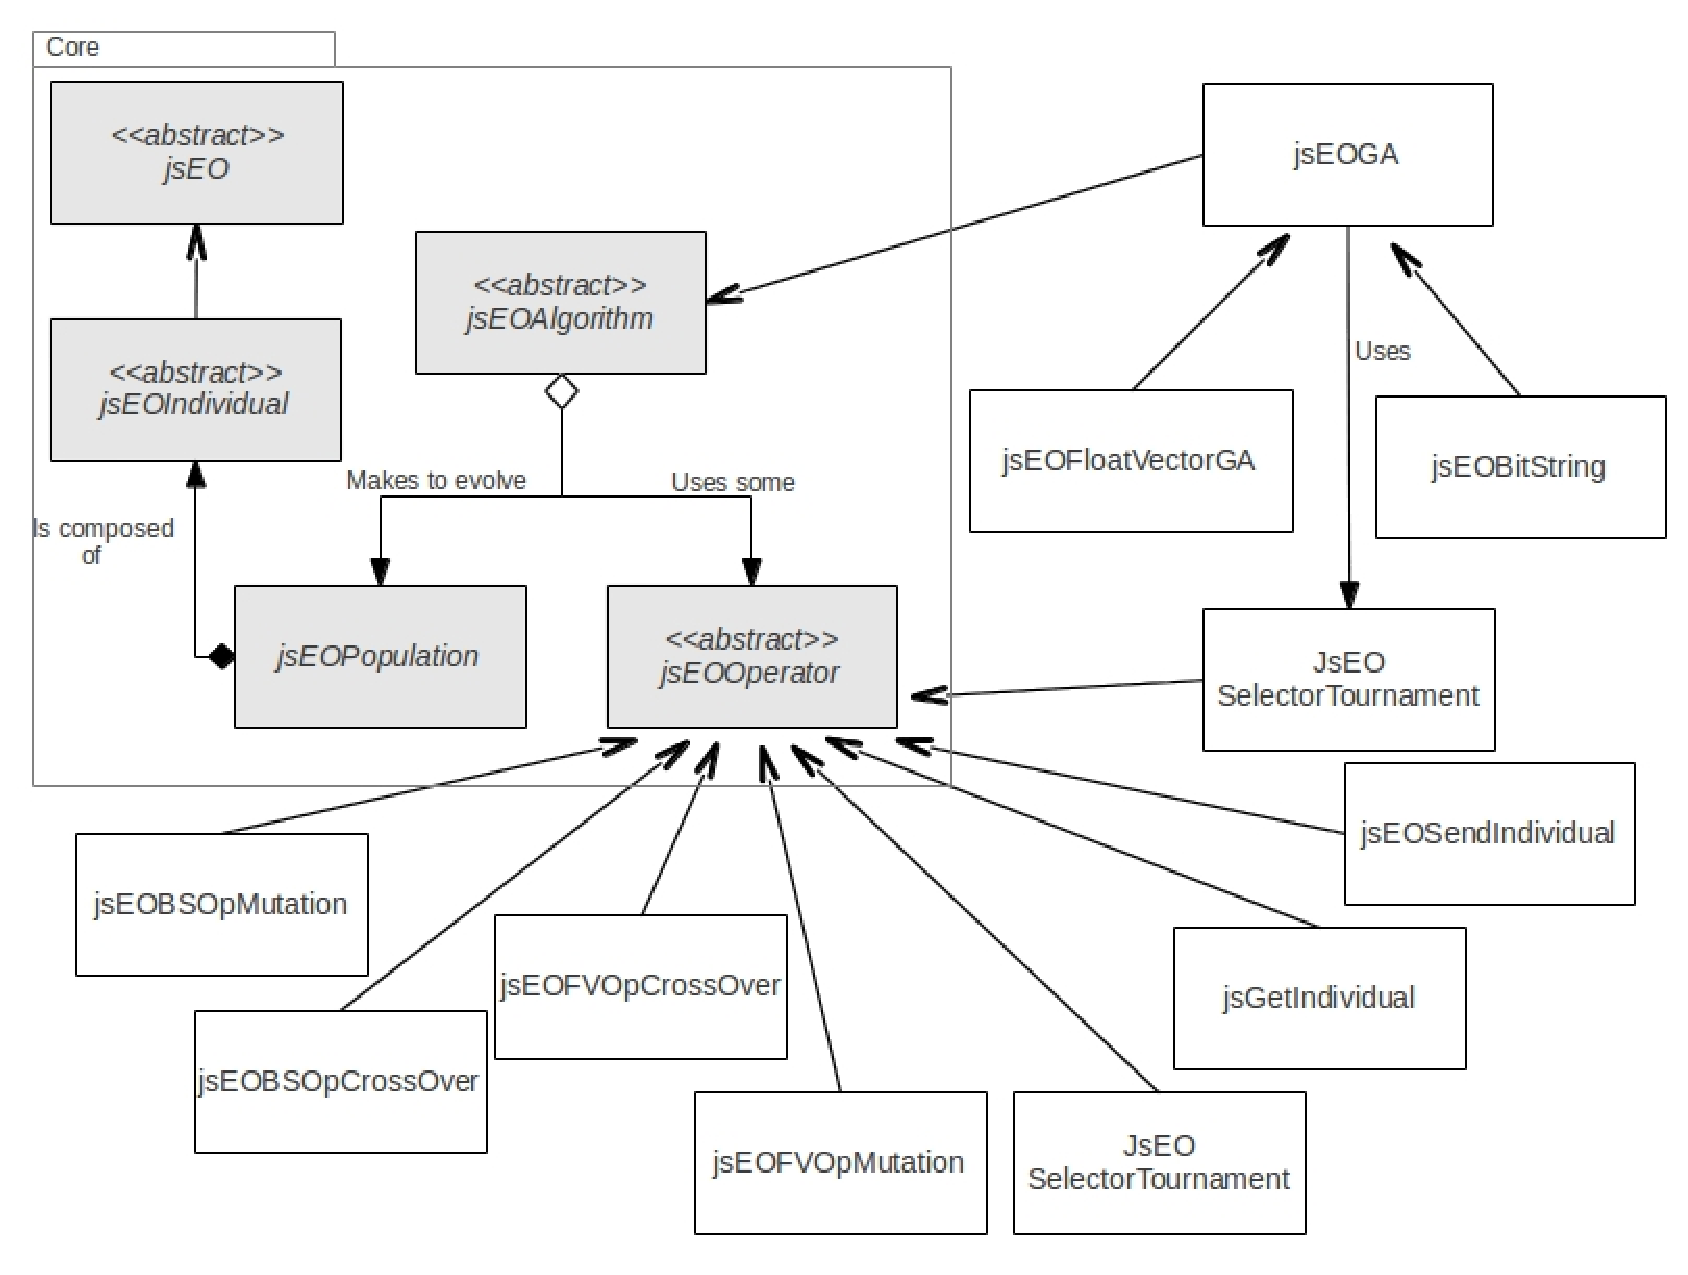
\includegraphics[height=10cm]{class-diagram}
\caption{Class diagram of jsEO. The core package include some abstract classes (\textit{jsEO, jsEOIndividual}, \textit{jsEOAlgorithm}, and \textit{jsEOOperator}) that make easier to develop new evolutionary algorithms by means of inheritance.}
\label{fig:jsEO-class-diagram}
\end{figure}


\section{Methodology and Experimental Setup}
\label{sec:method}
The experiments designed to the test jsEO include two problems, being the first the 256-bit Royal Road function, while the second is solving a 128-terms linear equation. In others words, the first one is related to a bit-string chromosome problem, while the second deals with vector of floats. Both problems have been executed as synchronized tasks, and are available at \url{http://jseo.vrivas.es}. Currently, synchronizing is quite constrained since it is done by means of AJAX connections to a server, without allowing to perform requests from pages hosted on a different one. 

Asking for collaboration to run the experiments was done publishing some messages in social nets as Facebook and Twitter, as well as sending an email to a group of about 70 computer-scientist professionals. The user who wanted to participate in the experiments only had to load in his/her browser a web file containing a brief description of the problem and the Javascript library, and the chosen problem was automatically executed. Users were able to select the problem they wanted to execute, to execute it as many time as desired, to change the problem at any moment, and, of course, to stop the execution by closing the browser or loading a new web page.

In order to execute every problem, two new classes were derived from class \textit{jsEOGA}, the first one to deal with bit-string chromosomes, the second one to make evolve vector of floats. The \textit{jsEOGA} is a steady state algorithm, with rank-based selection, and elimination of the worst individuals after joining the current population of every generation with the new individuals created by means of operators. The algorithm stopped after a given number of generations (table~\ref{tb:params} shows the parameters used), and incorporated operators for crossover and mutation. In the case of real problem, mutation consist on changing values for new random ones. After every generation, best individual was send to the server. On the other hand, requesting an individual to the server was done randomly according to the application rate of the corresponding \textit{jsEOGetIndividual} operator. Finally, two different evaluation functions were used, one per problem. In the case of 256-bit Royal Road function, the fitness corresponds to the number of "1111" or "0000" sequences found in the 256-length bit-string. In the case of 128-terms equation, the fitness was the inverse of the value obtained when evaluating eq.\ref{eq:128-term} with the 128 real values composing every chromosome.

Since both problems have been executed in a synchronous way, the best solution can be found in the server, but also in many clients as this individual is sent to the browser as soon as the \textit{jsEOGetInvididual} operator is selected to operate.



\begin{table}
\caption{Parameters used to run the experiments, as in{\cite{jj}}}
\begin{center}
\begin{tabular}{l@{\quad}rl}
\hline
\multicolumn{1}{l}{\rule{0pt}{12pt}
                   Parameter}&\multicolumn{2}{l}{Value}\\[2pt]
\hline\rule{0pt}{12pt}
Population size & 500 & \\
Tournament size & 2 & \\
Operator crossover's rate & 0.73 & \\
Operator mutation's rate & 0.18 & \\
Operator requesting individual's rate & 0.09 & \\
Number of genes affected by mutation & $1\%$ &\\
Individuals replaced in every generation & $50\%$ & \\
Range for new random real values && \\
(only for the 128-term equation problem) & $(-10,10)$ & \\[2pt]
\hline

\end{tabular}
\label{tb:params}
\end{center}
\end{table}

  	




\section{Experimental results}
\label{sec:exp}

After two days of volunteers executing the algorithms, some results can be drawn gathering data from the web server's log file (in this case, Apache log). The log file has been analysed using the free version of WebLog Expert application\footnote{WebLog Expert can be obtained from \url{http://www.weblogexpert.com/}}, and the well-known Webalizer application\footnote{Webalize can be obtained from \url{http://www.webalizer.com}}.

From a potential target of users of more than 500 people, the 128-terms equation has been executed 304 times by 231 different visitors, while the 256-bit Royal Road function has been executed 359 times by 279 visitors. Most of this visits (i.e., executions) were done along a period of approximately 24 hours, but no references about time consumed by every execution have been registered. The algorithms have been executed in up to 128 different combinations of web browser and operating system, any of them in many different versions. As shown in tables \ref{tb:browsers} and \ref{tb:operating-systems}, Web browser include Safari, Firefox, Chrome, Internet Explorer, and also native browsers for smartphones and tablets; while operating systems include Windows, Linux, MacOS, and Android.

\begin{figure}
\centering
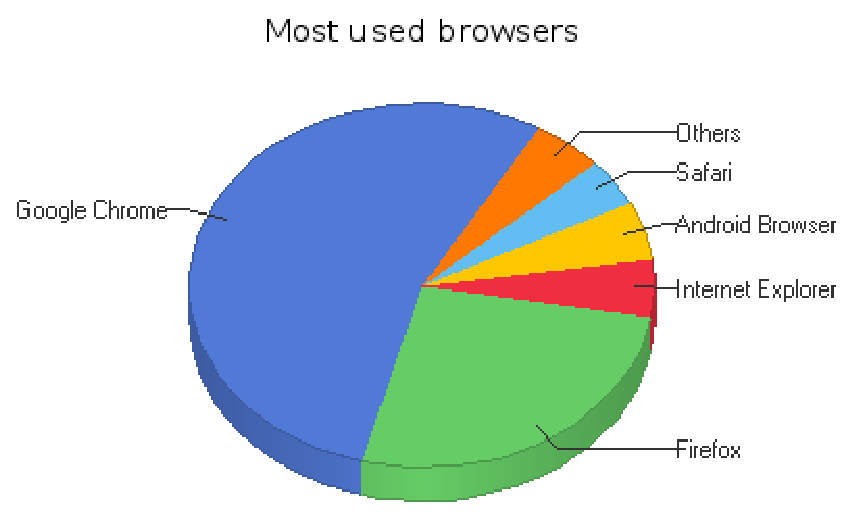
\includegraphics[height=5cm]{Most_Used_Browsers}
\caption{Summary of browsers used to run the experiments. For any of the browsers, many different versions have been used. For instance, up to 4 different versions of Internet Explorer were found.}
\label{fig:jsEO-str}
\end{figure}


\begin{figure}
\centering
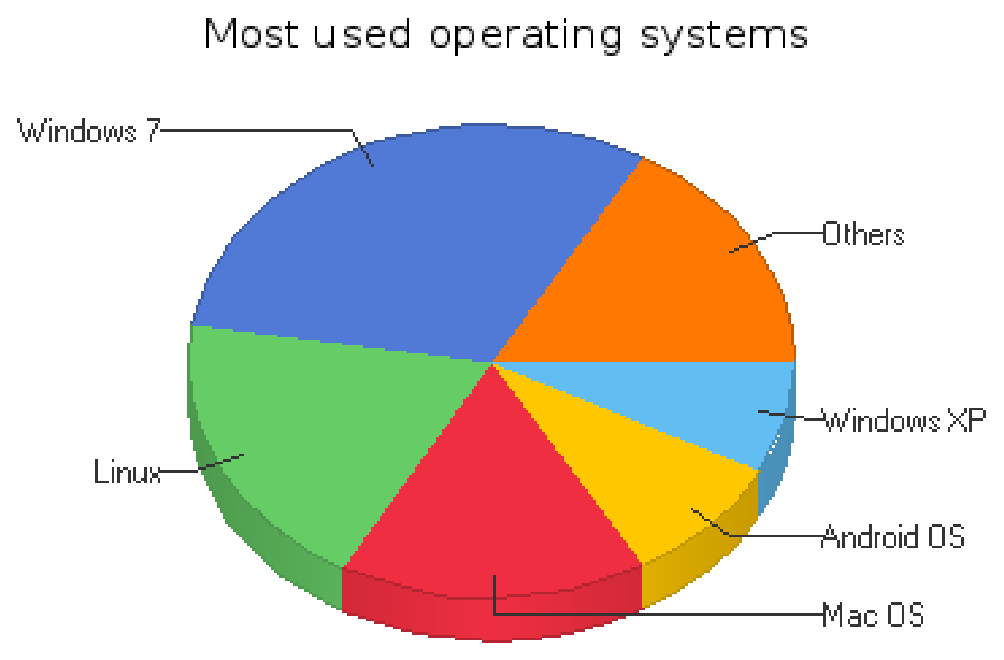
\includegraphics[height=5cm]{Most_Used_Operating_Systems}
\caption{Set of operating systems that have been used by users visiting the pages containing the experiments. The figures corresponding to Windows include 8 different versions, including the one for phones.
}
\label{fig:jsEO-str}
\end{figure}

As can be seen in table~\ref{tb:params}, population was composed by $500$ individuals, and $50\%$ were replaced in every generation, this means that in every execution $13,000$ individuals were evaluated. Consequently, the currently available solutions in the server have been found after $3,952,000$ evaluations in the case of the 128-terms equation, and $4,667,000$ evaluations for the 256-bit Royal Road function. The solution found for the bit-string problems is composed by 176 characters "0", and 80 characters "1", being  its fitness 232. For the real codified problem, the solution yields a fitness of $300,909.09$, which corresponds to a value of $3.32E-06$ when evaluating the equation being solved.

\section{Conclusions, discussion and future work}
\label{sec:conc}

While in previous papers  we proved that
this kind of AJAX based, volunteer, and potentially sneaky,
computation could be used profitably for performing genetic algorithm
experiments, in this paper we have proved that, 
without an expensive or far-fetched setup, it can achieve high
performance, equivalent, at most, to several computers of average
performance. The code used to perform the experiment is publicly
available and is modular so that creating different experiments is
just a matter of writing a new JavaScript fitness function and tuning
the GA parameters accordingly. 

The experiments have proved that there is a good amount of
computational power that can be easily tapped and used for
evolutionary computation experiments, however, the nature of jsEO
constrains also the way users donate computing power, as well as the
number of clients available for an experiment. In this paper we have
found some figures, which will undoubtedly vary for other experiments;
however, the general shape of the curves will probably be the same,
following a very steep decrease from the maximum values obtained. 

The GA, being asynchronous, faces some problems that have not been
tackled in this paper. What is the best approach to preserve
diversity? To generate a new population in each client, and receive
immigrants as soon as possible, which are incorporated into the
population? Or is it better to create new client populations based on
existing populations? What is really the algorithmic contribution of
new clients? These issues will be explored as future work. 
We will also try to measure the limits of this technology, and test
the impact of servers of varying performance and workload on overall
performance. Eventually, we will also try to perform a {\em sneaky}
experiment, to check what kind of performance can be expected in that
kind of setups. 

\section*{Acknowledgements}

Hidden for double-blind review

\bibliographystyle{unsrt}
\bibliography{evostar2007,GA-general,geneura,ror-js,volunteer}

% that's all folks
\end{document}
